\chapter{Android}\label{sec:Android}
This chapter will provide information about Android and WearOS technology from the same company. Why it was developed and what are the differences between previous versions and other wear technologies.

Android is a Linux based operating system for mobile and wear devices developed by Google. The main selling point of this system is being an open-source project, meaning everyone can access the code and modify it as they wish. Android was mainly developed for mobile platform but in time moved beyond and can be implemented into all kinds devices, such as wear, tablets, televisions and even refrigerators or cameras \cite{WIGA}.

\section{Android system structure}\label{sec:AndroidSystemStructure}
Android is created as a stack, meaning there are functional modules \enquote{stacked} on top of each other from Linux core over native libraries to applications as shown in \fref{fig01c04}.

\begin{figure}[H]
	\begin{centering}
		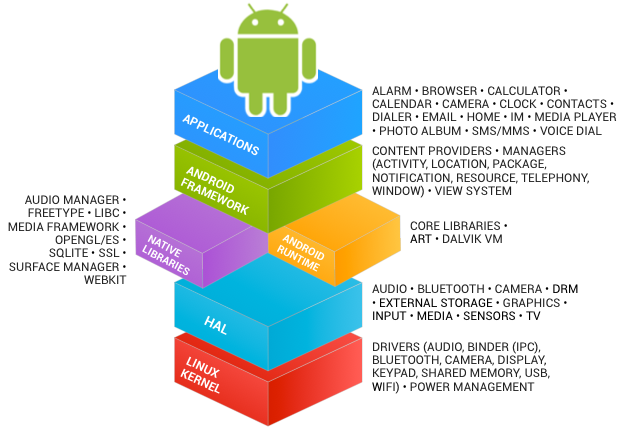
\includegraphics[width=0.6\textwidth]{img/android_stack}
		\par\end{centering}
	\caption{Android stack (source: \cite{AOSP})\label{fig:AndroidStack}}
	\label{fig01c04}
\end{figure}

Android maintains all implementations with complete software stacks to enable device creators to run and modify Android for their specific hardware. To support these modifications and testing every release has multiple \enquote{code lines} to separate stable versions from experimental work \cite{AOSP}. There are multiple versions of Android system at this time and every single one has its own version information, code name and API level. Version codes are number identifications of a specific system build. Highest levels of these numbers are grouped into code names that are ordered alphabetically. For example, versions 8.0.0 and 8.1.0 have both the same code name called Oreo. Finally API level is number identification for compatibility of specific application and is always compared to API level of device Android system \cite{AOSP, AD}. Devices with API levels lower than minimum level supported by the application are not able to run it.

The highest part of the Android system stack are applications which extend device functionality and are written primarily in Java or newly supported Kotlin programming language \cite{SoASTaD}. These application files are packaged into \textbf{.apk} file, which is a zip archive, containing all application files like Java classes, layouts, images and more. One of the very important files is \textbf{AndroidManifest.xml}, it contains all meta-data about the application, such as permissions, package name, used components, versions and so on. These application packages can be shared, for a nominal fee, via official Android market called Google Play. At the end of 2017 there were over three and a half million applications available in Google Play Store \cite{SoASTaD, NoAAiGPS, NoAA}.

Application permissions maintain security for the system and users. Android requires that application declares the permissions it needs before it can use certain system data and features. Depending on how sensitive the area is, the system may grant the permission automatically, or it may ask the user to approve the request. Following example shows how to set required application permissions in AndroidManifest, Internet is granted automatically but location must be manually approved by device user.

\begin{lstlisting}[caption=Application permission settings]
<uses-permission android:name="android.permission.INTERNET" />
<uses-permission android:name="android.permission.ACCESS_FINE_LOCATION" />
\end{lstlisting}

Android is a platform designed to be open-source and free which also makes it easy to create malicious applications. These application can bypass existing security and steal sensitive data, use telephone services or even gain control over the device \cite{ASIMPD}. Android has multiple ways to protect against such applications one of the most notable ones are Android Permission Framework and Google Play Protect \cite{SoASTaD}.

\section{Wear technologies}\label{sec:WearTechnologies}
Interactive wearable, as an example smartwatches, is a new part of mobile computers. Wear devices are categorically different from mobiles or tables in terms of usage, look and user interfaces (UI). According to the application design guidelines from major vendors users interact with wearable devices frequently throughout daily use. Each interaction is short, often less than 10 seconds, and dedicated to complete simple tasks \cite{UtCoAWO}. 

Important thing to note is that there are multiple kinds of wear devices from watches, wristbands, cameras or even glasses \cite{MIWD}. Based on a report from Gartner technology research, conducted in 2017, most used wear devices were Bluetooth headsets, wristbands and smartwatches, in this order \cite{GSWWDS}. Thanks to their small size, wear devices are ideal to use for hands-free communication and health monitoring.

One problem of these devices is their diversity in hardware and more importantly in software compatibility. Every device manufacturer can create their own operating system for specific wear device and it can be difficult to develop custom applications for them. To avoid such problems this thesis is focused only on smartwatch with WearOS operating system which is based on Android. 

There are three main points to mention considering wear devices. First, small battery capacity that can be almost ten times smaller than of typical smartphone. Second, small display size with around forty-times less pixels which completely changes its properties. Finally, scaled down CPU with high efficiency \cite{UtCoAWO}. Last two points are main parts of lowering power consumption of smartwatches but even with these cuts high-end watch devices can have really small battery life only in matter of few days or even hours.

\subsection{WearOS by Google}\label{sec:WearOS}
WearOS by Google, formally known and Android Wear 2.0, is a version of Android operational system tailored to small-screen wearable devices. There are not too many in-system changes from smartphone but one of the main differences can be seen in UI since system had to be adjusted for watch size \cite{CSUITW}. Due to scaled down processing power of watches can offload data wirelessly to mobile for heavy computing tasks, e.g. voice recognition \cite{UCAW}.

\begin{figure}[H]
	\begin{centering}
		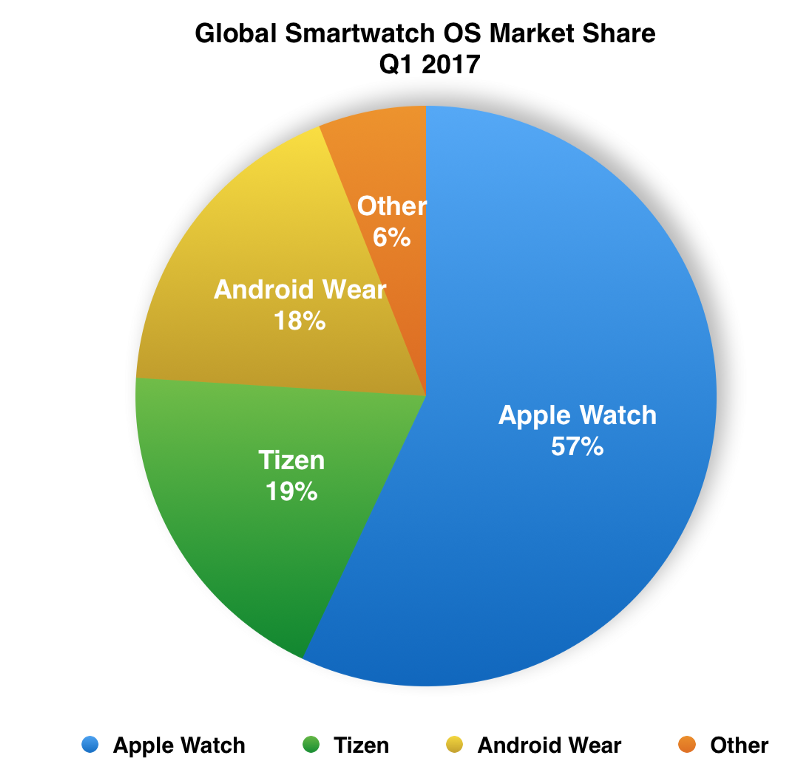
\includegraphics[width=0.6\textwidth]{img/wear_market_share}
		\par\end{centering}
	\caption{Smartwatch OS market share (source: \cite{TOAW})\label{fig:SmartwatchOSMarketShare}}
	\label{fig02c04}
\end{figure}

WearOS is one of the three most popular smartwatch systems but it comes with its own set of problems. Most notable and annoying one is being unable to pair wear with specific mobile device. It can be caused by multiple reasons, such as system compatibility, custom hardware or mobile type and it is more common than it should be \cite{AWPaS}. Having smartphone connected to WearOS can also cause faster battery drain on mobile device. Important thing to mention is that smartwatch can be connected to only single device and connecting to another mobile requires watch factory reset. Some other problems can be: software update issues, notifications not coming through to the watch, not being able to connect to WiFi, system crashes and few more \cite{WAWP}.

Even with all these problems it is popular system and in early 2017 it got its biggest update yet. New version 2.0, later renamed to WearOS, which brought numerous improvements and features where few of the most notable ones will be described in this section \cite{AW2UG, AW2WN, AW2N}.

\subsubsection{Standalone applications}\label{sec:StandaloneApplications}
This feature is a crucial change and enables smartwatch applications to run without the need for mobile device to be constantly connected. Before this version it was needed to have smartphone connected to Android Wear when application was supposed to be used. It also supported only connection to Android device and that proved as an obstacle for users without one since they could not use any applications on the watch \cite{AW2UG, AW2WN}.

This change made applications work without mobile and also created the need for them to be installed directly on wear without the need for controlling device. Thankfully part of this update is also standalone Google Play Store where users can browse applications that are designed specifically for the smartwatch \cite{AW2WN}. Part of this feature is also enabling watch to use wireless and cellular networks on their own since most standalone applications require at least WiFi connection. Finally, as of this update, security for communicating between wear and mobile was reworked and improved. Communication is now done via Wearable Data Layer API that is used in almost all Google applications and it is also easy to use for a developer \cite{AW2UG}. 

\subsubsection{UI improvements}\label{sec:UIImprovements}
Part of new Android Wear version is implementation of Android's Material design guidelines \cite{DoAW}. It has much more \enquote{mature} look and darker design for reducing battery drain \cite{AW2WN}. It is completely focused on wear devices and supports both round and square screens with new re-design of application launcher \cite{AW2UG}.

\begin{figure}[H]
	\begin{centering}
		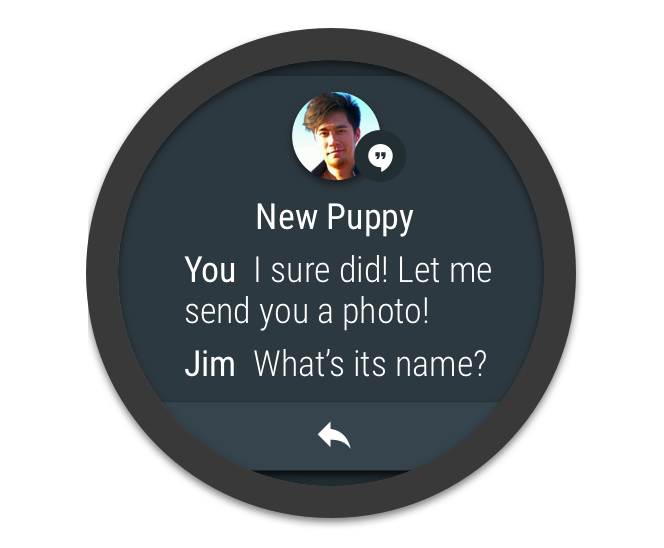
\includegraphics[width=0.3\textwidth]{img/wear_design_notification}
		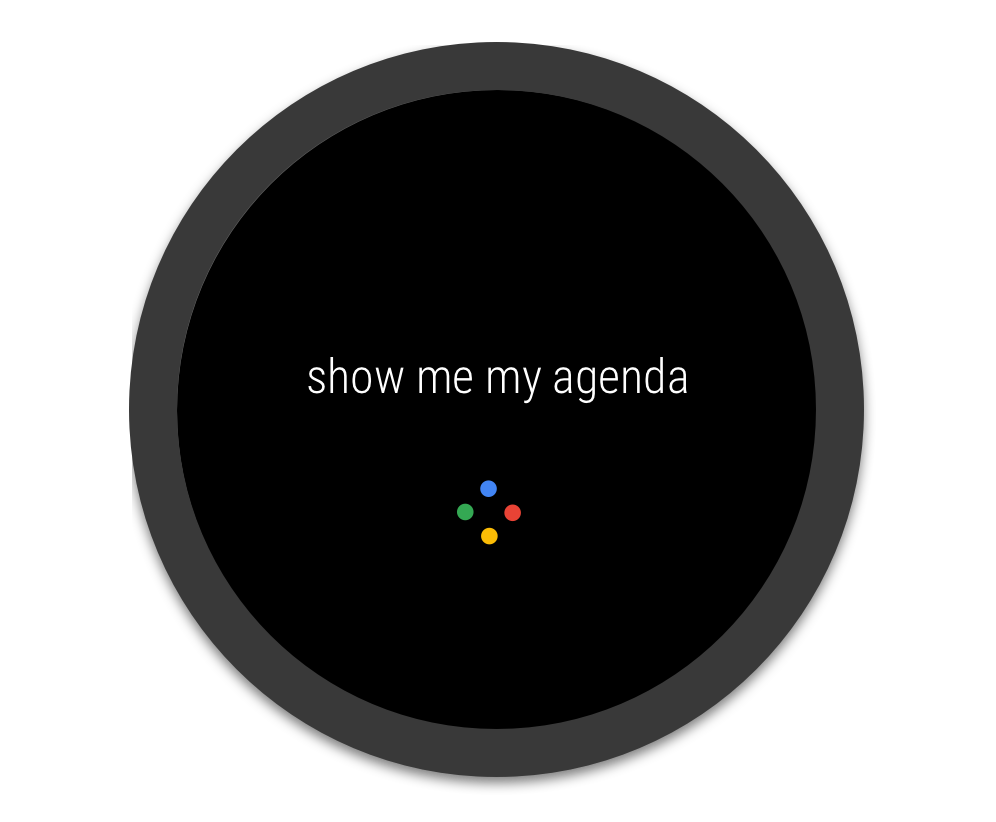
\includegraphics[width=0.3\textwidth]{img/wear_design_agenda}
		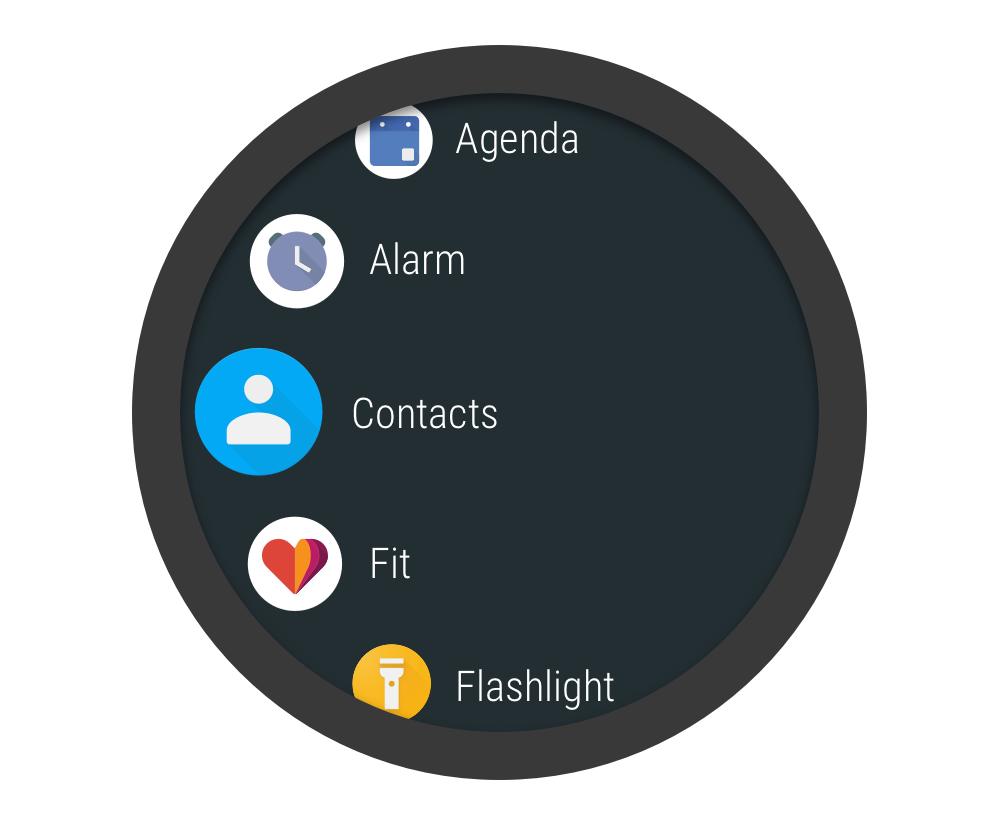
\includegraphics[width=0.3\textwidth]{img/wear_design_menu}
		\par\end{centering}
	\caption{Wear design examples (source: \cite{DoAW})\label{fig:WearDesignExamples}}
	\label{fig03c04}
\end{figure}

Android is also trying to catch up with Apple's watchOS and that is why they remade default watch display, also called watch faces, and made it much more useful. Users can now add different widgets with data from any application to the watch faces \cite{AW2UG}. This ensures quick access to the information user deems important \cite{AW2N}. All this data displays also match design of currently selected watch face and after clicking it user is directed right into the application \cite{AW2WN}.

\begin{figure}[H]
	\begin{centering}
		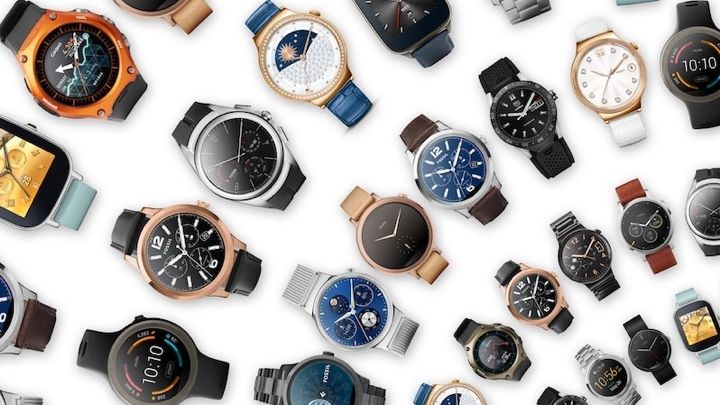
\includegraphics[width=0.5\textwidth]{img/wear_watch_faces}
		\par\end{centering}
	\caption{Wear watch faces (source: \cite{AW2UG})\label{fig:WearWatchFaces}}
	\label{fig04c04}
\end{figure}

\subsubsection{Google Assistant}\label{sec:GoogleAssistant}
Google Assistant is basically voice controlled smart assistant, such as Amazon's Alexa, Apple's Siri or Microsoft's Cortana. There are multiple tech sites that run benchmarks of these systems \cite{ASGA, VACCGASAB, CAGACS, GASBAC} and there are not too many differences between them so no actual need to buy one over the other. These systems can pull information that user needs or wants and these systems also track important information like place of work, sport interests, daily schedule, data related to health and much more \cite{WIGA}. With the update of WearOS this assistant is now also available on smartwatches \cite{AW2UG, AW2WN}.

\section{Other wear technologies}\label{sec:OtherWearTechnologies}
During the first years of smartmatches big amount of manufacturers created their own operating systems and flooded the market with them but that was a long time ago and situation has changed since then. Now there are only three main competitors as shown in the \fref{fig02c04} and those are Android (WearOS), Samsung (Tizen) and Apple (WatchOS). System from Android was already introduced so it is time for Tizen and WatchOS.

\subsection{Tizen}\label{sec:Tizen}
Between year 2010 and 2012 there were multiple companies developing different wear systems like MeeGo by Nokia and Intel, Samsung Linux Platform (SLP) or Bada created by Samsung. Intel later decided to join forces with Samsung and they created Tizen organization and project which was based on SLP. This project either canceled support of previous systems or merged with them \cite{TOSBHR}. Some of the current members of Tizen organization are: Samsung, Intel, Huawei, Vodafone or SK Telecom \cite{TizenM}.

Tizen system is built from the ground up on Linux platform and is a part of Linux Foundation. It is focused on the needs of all stakeholders of the mobile and connected device ecosystem based on the hardware on which it should run, such as mobile, tv and wearable. One of this systems main focuses is easy support for different manufacturers by using easily changeable profiles to suit the needs of a specific manufacturer. Tizen also offers the power of native code development with the flexibility of unparalleled HTML5 support \cite{TizenAbout}.

\begin{figure}[H]
	\begin{centering}
		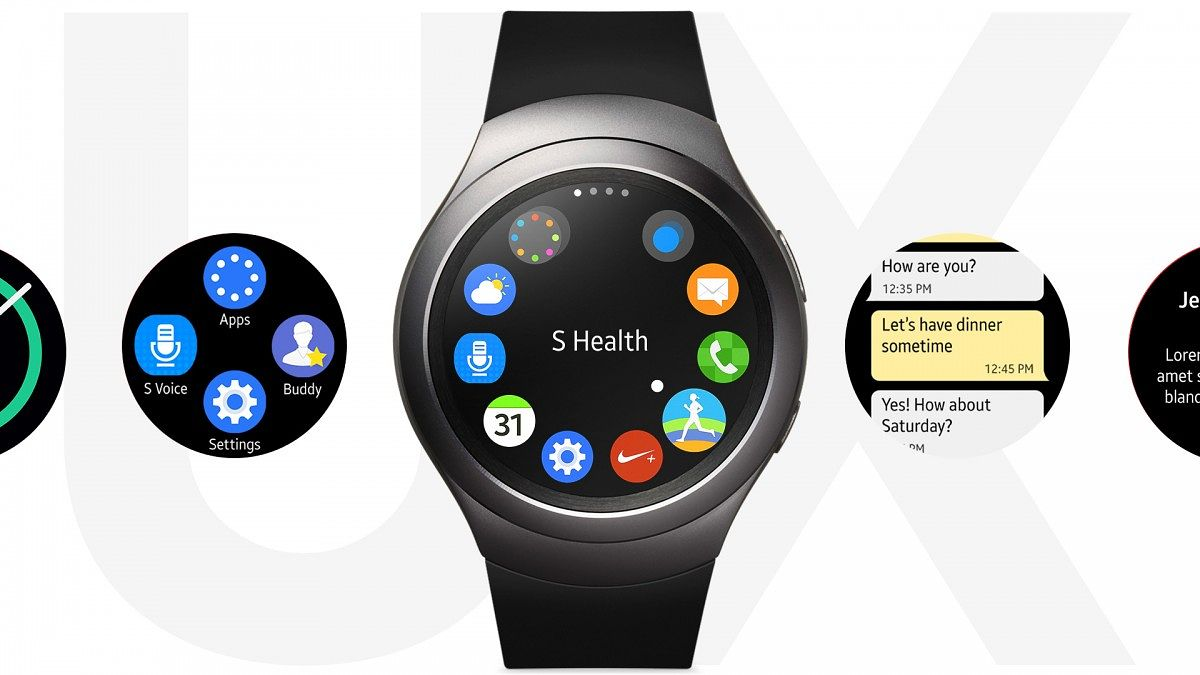
\includegraphics[width=0.6\textwidth]{img/tizen}
		\par\end{centering}
	\caption{Tizen showcase (source: \cite{NFFAWSW})\label{fig:Tizen}}
	\label{fig05c04}
\end{figure}

Developing application for this system can be done in a custom made program Tizen Studio which supports developing native or Web applications where native apps are developed using the C programming language, but since Tizen version 4.0 application can also be developed using .NET or Xamarin UI. This studio contains all required part for developing an application from project management, writing and editing code, debugging and running the application. Newest version of Tizen Studio is 2.3 with the support of Windows, Ubuntu and macOS where the next version will remove support for 32-bit Windows and Ubuntu. Created applications can be deployed to Taizen store which is very similar to Google Play for Android system \cite{TizenDev}.

Even though wear version of Tizen OS is deployed only on Samsung products it overtook Android Wear in market shares in the beginning of 2017 but that might change with the release of Android Wear 2.0 (WearOS). 

\subsection{WatchOS}\label{sec:WatchOS}
Apple started working on smartwatches around year 2002 inspired by sportswatches from Nike, with the actual results few years later (2014), when Apple Watch was revealed to be released in 2015. The release of this smatwatches introduced a new version of iOS system focused solely on wear devices called watchOS. Compared to previously mentioned systems this one is the youngest but most popular of them \cite{ATOHAWWC}. WatchOS is currently developed and deployed only for Apple Watches, same as Tizen for Samsung devices, making Google's WearOS only of them to be implemented by multiple wear manufacturers. First version of watchOS was based on the same principle as Android Wear because it required mobile device to use its applications but luckily for Apple, they quickly moved from this interaction in version 2.0. Next versions brought many improvements, such as running application in the background, improved design and support of completely mobile independent application in the newest major version 4.0 \cite{WOS9To5MAC}.

Applications of this system consist of two related bundles: Watch app and WatchKit extension. The Watch app bundle contains the storyboards and resource files associated with application's user interfaces. The WatchKit extension bundle lives inside the Watch app and contains the code for managing those interfaces and for responding to user interactions \cite{AppleDev}.

\begin{figure}[H]
	\begin{centering}
		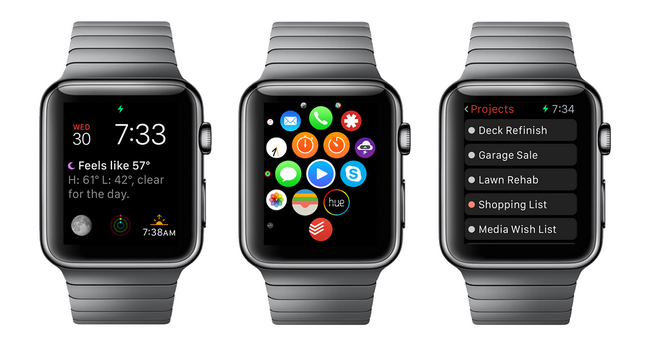
\includegraphics[width=0.6\textwidth]{img/apple_watchOs}
		\par\end{centering}
	\caption{WatchOS showcase (source: \cite{HTFAIAAW})\label{fig:WatchOS}}
	\label{fig06c04}
\end{figure}

Application development for WatchOS can be done using Xcode which is a free program to develop applications for iOS platform created by Apple. Main programming language used in this program is Swift, also created by Apple and based on C and Object-C language. Swift is an open-source language focused on being easy to understand but still powerful and fast. Same as previous wear systems, created applications can be deployed using an App Store similar to Google Play or Tizen store.